\section{Regresión Logística (logit)}
\label{resultados:lr}

\subsection{Características de los conjuntos de datos a analizar}
\label{resultados:lr_caracteristicas}
Al realizar las mismas transformaciones que para el caso de \hyperref[resultados:knn_caracteristicas]{K-NN}, las características de los conjuntos de datos son las mismas.

\subsection{(Caso de estudio 1) Resultados del entrenamiento con el Conjunto de datos solo con atributo utilidad definido y escogiendo los atributos que nos ha indicado como relevantes el \hyperref[result:pca_case2]{caso de estudio 2} del PCA}

\paragraph{}
Realizamos el entrenamiento del modelo de Regresión Logística\cite{ref:lr_def} y aplicamos una validación cruzada\cite{ref:lr_cross_validation} para valorar su precisión. Este nos muestra una \textbf{precisión de cerca del 51\% con una desviación estándar de casi el 28\%}, lo que nos indica que el modelo tiene una precisión baja. Al realizar la predicción \textbf{sobre el conjunto de validación}, este nos da \textbf{una precisión del 65\%}. Lo que nos confirma que el modelo \textbf{tiene una precisión muy baja} (llegando casi al nivel de la aleatoriedad). Puede consultar los pasos realizados para el entrenamiento del modelo en el anexo (\nameref{anx04:rl1}).

\paragraph{}
Si mostramos la matriz de confusión\cite{ref:confusion_matrix} (figura \ref{lrCMCase1}) para poder ver que porcentaje de aciertos tiene el modelo con el conjunto de test, confirmamos que el porcentaje de aciertos es bajo.

\subsection{(Caso de estudio 2) Conjunto de datos solo con atributo utilidad definido, añadiendo el mes y año del artículo, eliminando los atributos \textit{gender} y artículo y expandiendo el atributo \textit{respuesta.pubmed\_keys}. También escogemos solo los atributos que nos ha indicado como relevantes el \hyperref[result:pca_case3]{caso de estudio 3} del PCA}

\paragraph{}
Igual que para el caso anterior realizamos el entrenamiento y aplicamos la validación cruzada para valorar su precisión. Este nos muestra \textbf{una precisión aun menor que para el caso de estudio 1 (49\%)}. Puede consultar los pasos realizados para el entrenamiento del modelo en el anexo (\nameref{anx04:rl2}).

\paragraph{}
Si mostramos la matriz de confusión\cite{ref:confusion_matrix} (figura \ref{lrCMCase2}) para poder ver que porcentaje de aciertos tiene el modelo con el conjunto de test, podemos ver con suficiente claridad que el \textbf{porcentaje de aciertos es muy bajo}.

\begin{figure}[!htb]
    \begin{subfigure}[b]{0.45\linewidth}
    	\centering
    	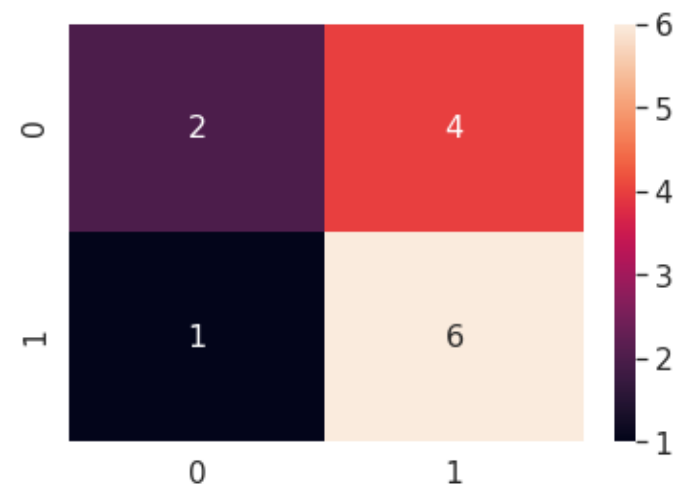
\includegraphics[width=0.9\textwidth]{images/resultados_lr_cm_conjunto1.png}
		\caption{Matriz de confusión para el modelo Regresión Logística en el caso de estudio 1.}
		\label{lrCMCase1}
	\end{subfigure}
	\begin{subfigure}[b]{0.45\linewidth} 
		\centering
	    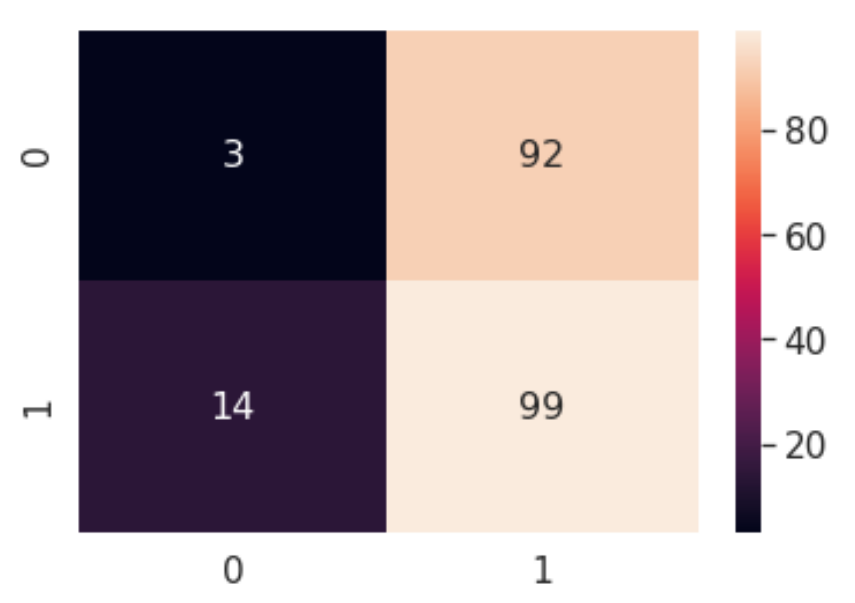
\includegraphics[width=0.9\textwidth]{images/resultados_lr_cm_conjunto2.png}
		\caption{Matriz de confusión para el modelo Regresión Logística en el caso de estudio 2.}
	  \label{lrCMCase2}
	\end{subfigure}
	\caption{Matriz de confusión para el modelo Regresión Logística.}
	\label{lrcm}
\end{figure}

\subsection{Conclusiones del modelo de Regresión Logística}
\label{resultados:lr_conclusiones}

\paragraph{}
Después de realizar el entrenamiento y posterior validación de los modelos podemos \textbf{desaconsejar su uso debido a su bajo porcentaje de aciertos}. Es posible que con un volumen de datos superior este se pueda comportar mejor, pero no se da el caso con el conjunto de datos que tenemos en la actualidad.
